\documentclass[../hw4]{subfiles}
\begin{document}
\begin{problem}
Are the following two graphs isomorphic?

\begin{center}
	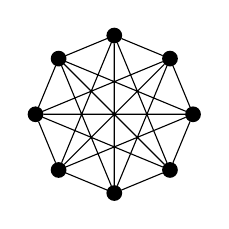
\begin{tikzpicture}[vertex/.style={circle, fill, minimum size=2mm, inner sep=0mm, outer sep=0mm}]
		\node[vertex] at (0:1) (1) {};
		\node[vertex] at (45:1) (2) {};
		\node[vertex] at (90:1) (3) {};
		\node[vertex] at (135:1) (4) {};
		\node[vertex] at (180:1) (5) {};
		\node[vertex] at (225:1) (6) {};
		\node[vertex] at (270:1) (7) {};
		\node[vertex] at (315:1) (8) {};
		\draw (1)--(2)--(3)--(4)--(5)--(6)--(7)--(8)--(1)
		(1)--(4)--(7)--(2)--(5)--(8)--(3)--(6)--(1) (1)--(5) (2)--(6) (3)--(7) (4)--(8);
	\end{tikzpicture}
	\qquad\quad
	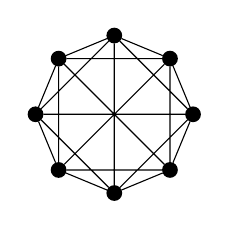
\begin{tikzpicture}[vertex/.style={circle, fill, minimum size=2mm, inner sep=0mm, outer sep=0mm}]
		\node[vertex] at (0:1) (1) {};
		\node[vertex] at (45:1) (2) {};
		\node[vertex] at (90:1) (3) {};
		\node[vertex] at (135:1) (4) {};
		\node[vertex] at (180:1) (5) {};
		\node[vertex] at (225:1) (6) {};
		\node[vertex] at (270:1) (7) {};
		\node[vertex] at (315:1) (8) {};
		\draw (1)--(2)--(3)--(4)--(5)--(6)--(7)--(8)--(1)
		(1)--(3)--(5)--(7)--(1) (2)--(4)--(6)--(8)--(2) (1)--(5) (2)--(6) (3)--(7) (4)--(8);
	\end{tikzpicture}
\end{center}
\end{problem}
\begin{proof}
	Since isomorphism preserves all structured properties of a graph, then we first note that both graphs have all 8 vertices of degree 5, and therefore also both have 20 edges.

	Since both graphs have their vertices arranged in the same way, we can expose the differences in each graph by removing edges that are the same.

	Now, we have
	\begin{center}
		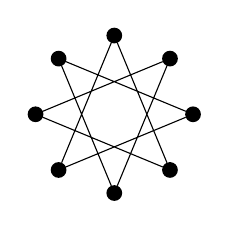
\begin{tikzpicture}[vertex/.style={circle, fill, minimum size=2mm, inner sep=0mm, outer sep=0mm}]
			\node[vertex] at (0:1) (1) {};
			\node[vertex] at (45:1) (2) {};
			\node[vertex] at (90:1) (3) {};
			\node[vertex] at (135:1) (4) {};
			\node[vertex] at (180:1) (5) {};
			\node[vertex] at (225:1) (6) {};
			\node[vertex] at (270:1) (7) {};
			\node[vertex] at (315:1) (8) {};
			\draw
			(1)--(4)--(7)--(2)--(5)--(8)--(3)--(6)--(1);
		\end{tikzpicture}
		\qquad\quad
		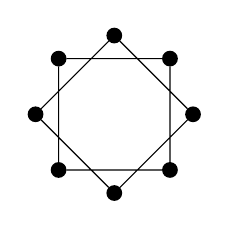
\begin{tikzpicture}[vertex/.style={circle, fill, minimum size=2mm, inner sep=0mm, outer sep=0mm}]
			\node[vertex] at (0:1) (1) {};
			\node[vertex] at (45:1) (2) {};
			\node[vertex] at (90:1) (3) {};
			\node[vertex] at (135:1) (4) {};
			\node[vertex] at (180:1) (5) {};
			\node[vertex] at (225:1) (6) {};
			\node[vertex] at (270:1) (7) {};
			\node[vertex] at (315:1) (8) {};
			\draw
			(1)--(3)--(5)--(7)--(1) (2)--(4)--(6)--(8)--(2);
		\end{tikzpicture}
	\end{center}

	But, we see that the left graph has one 8 cycle, while the right has two 4 cycles.
	Since these graphs do not have the same number of cycles, then they are not isomorphic.
\end{proof}
\end{document}
